\documentclass{standalone}
\usepackage{tikz}
\usepackage{amsmath}
\usetikzlibrary{positioning}
\usetikzlibrary{arrows,automata} 

\tikzset{main node/.style={circle,,draw,minimum size=1cm,inner sep=0pt} }
\begin{document}

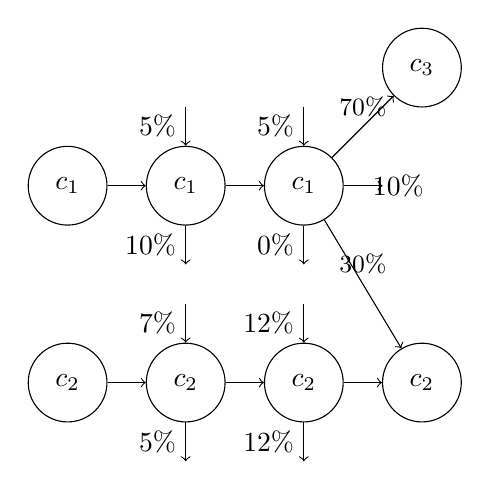
\begin{tikzpicture}
\begin{scope}[on grid]

  \node[main node] (1) {$c_1$};
  \node[main node] (2) [ right =1.5cm of 1] {$c_1$};
  \node[main node] (3) [right =1.5cm of 2] {$c_1$};
  
  \node[main node] (4) [below =2.5cm of 1]{$c_2$};
  \node[main node] (5) [right =1.5cm of 4] {$c_2$};
  \node[main node] (6) [right =1.5cm of 5] {$c_2$};
  \node[main node] (7) [right =1.5cm of 6] {$c_2$};
  
  \node[main node] (8) [above right =1.5cm  and 1.5cm of 3] {$c_3$};

    \path[every node/.style={font=\sffamily\small}]

    (1) edge [->] (2)
    (2) edge [->] (3)
    (3) edge [->] node[above] {$30\%$}(7)
    (3) edge [->] node[above] {$70\%$}(8)
    
    (4) edge [->] (5)
    (5) edge [->] (6)
    (6) edge [->] (7)
    ;
     \draw [->] (2) to[left] node[left] {$10\%$} ++ (0,-1);
     \draw [<-] (2) to[left] node[left] {$5\%$} ++ (0,1);
     
     \draw [->] (3) to[left] node[left] {$0\%$} ++ (0,-1);
     \draw [<-] (3) to[left] node[left] {$5\%$} ++ (0,1);
     \draw [->] (3) to[left] node[right] {$10\%$} ++ (1,0);
     
     \draw [->] (5) to[left] node[left] {$5\%$} ++ (0,-1);
     \draw [<-] (5) to[left] node[left] {$7\%$} ++ (0,1);
     
     \draw [->] (6) to[left] node[left] {$12\%$} ++ (0,-1);
     \draw [<-] (6) to[left] node[left] {$12\%$} ++ (0,1);
    \end{scope}
\end{tikzpicture}
\end{document}